\documentclass[class=article, crop=false]{standalone}
\usepackage{graphicx}
\graphicspath{{../Figures}}
\usepackage{rotating}
\setkeys{Gin}{width=0.9\textwidth}

\usepackage{cleveref}

\begin{document}
There are three elements that will be discussed here: results and development of the simulator, results and development of the control system

\section{Simulated cases}
The goal of the simulated scenario is to show whether the simulator and the control system are suitable for the purpose of controlling the vessel. The results shown so far are promising but indicate that they are not.

As mentioned early in \cref{sec:case} several more cases were simulated but their data has been discarded from this discussion. Originally the goal for simulation was to simulate only 0m, 1m and 2m waves, but this was expanded to include also 0.5m and 1.5m waves. This turned out to be a good thing, as the simulation does not do well with waves above 1m in height. There are two criteria that the system does not meet in higher waves. The first is vessel stability, the second is controllability.

When it comes to vessel stability, the vessel capsizes very easily at higher wave heights. No direct data has been gathered on this, but it is visible in the simulator viewport. See \cref{fig:half_capsized} for an example of this. It's not unreasonable that the vessel struggles with large waves as it is fairly small. The length of the vessel implemented here is approximately 2.8m long and 3m wide. Comparing this size to a 2m wave, it makes intuitive sense that the vessel is unstable in those situations.

\begin{figure}
    \centering
    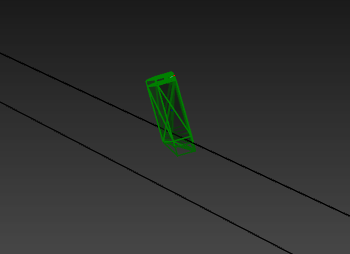
\includegraphics{2m-wave-half-capsized}
    \caption{The vessel experiencing a 2m wave almost capsizing}
    \label{fig:half_capsized}
\end{figure}

Another possible contributor to this easy capsizing is that the vessel is currently simulated uniformly dense. This is unrealistic and a limitation of the current simulation. A real vessel is almost always heavier near the keel than near the deck, as this provides greater stability. For this vessel in particular, the hull and deck are made from lightweight carbon fiber boards, while heavy batteries and ballast will be placed low down in the hulls. This would make it so the large flat deck is nowhere near as dense as the lower hulls, and would hopefully shift the center of gravity down towards the keels and help with stability. It is possible to implement density gradients and non-uniformly dense materials in AGX, and this should be considered as a future addition.

With regards to controllability, the results (especially \cref{fig:fucked_position}) demonstrate how the vessel is not capable of controlling itself in the simulated scenario. It looks from the results like the power allowed for the vessel is too low, meaning that it is not able to withstand the external forces placed upon it. The vessel drifts even in low waves, see \cref{fig:1.0m-controlled}. Another example of low authority is the torque curves, \cref{fig:torque}. These reach saturation very quickly in most situations, meaning that they no longer are able to control the vessel any more than they already are. The issues with command authority stem from improper assumptions made about the vessel's capability, as well as the quite violent situations that the vessel is placed in.

Even discounting insufficient command authority, it is clear that the controller is still not functioning as desired. This can be seen in the wave-less cases, such as below in \cref{fig:nowaves}. The vessel is moving around in these large circles. The same is seen in the 0.5m wave cases, though less clearly due to the drift of the vessel. This shows that the system is improperly tuned. The same tuning issues can be seen in the heading control results, where there is a constant oscillation about the setpoint. Luckily, these issues are solved with higher command authority and controller tuning.

\begin{figure}
    \centering
    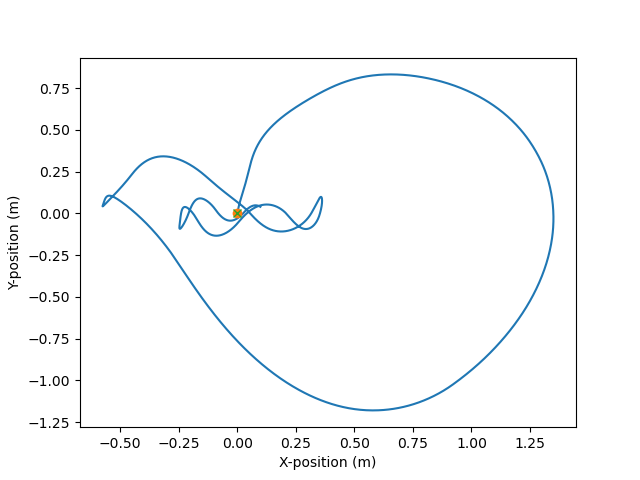
\includegraphics{scenario1/rov-50m/0.0m/usv_position_controlled}
    \caption{The position of the USV in no waves with ROV at 50m}
    \label{fig:nowaves}
\end{figure}

\subsection{On the subject of seastate}
This simulation uses regular waves, meaning that the wave height at any point in space and time is defined by the wave height equation discussed in previous chapters. This is not realistic compared to a real-world seastate. Real-world seastates are random and complex. This makes them harder to simulate than regular waves, and also changes how they affect the vessel.

There is an argument for using a regular seastate in this sort of simulation. As the shape of the uncontrolled results shows, (\cref{fig:1.0m-uncontrolled}), the effect is predictable. The vessel in this current simulation setup will always move south-west when left adrift with wave forces. This is helpful for this kind of "stupid" (i.e. not a "learning") control system. Random effects won't be as prominent, and two different wave heights or control systems can be compared more easily. If the control system had machine learning implemented in some way, this regular seastate would be detrimental to the results. This is because the system would likely overfit to this specific kind of seastate and not be generalizable to other seas.

\subsection{On the subject of mastering}
One of the goals of this project has been to implement a reversibly mastered system, i.e. that both the surface vessel and the ROV can be the one "in charge" of deciding where to go. If the ROV is mastered, the USV attempts to follow, and the other way around. This has been implemented in the controllers for the USV and the ROV, but has not been tested in simulation. The way the mastering works is that if the vessel is mastered it recieves its target position from the operator, while if it's slaved it simply tries to match the position of the master vessel. In short: the system is currently mastered and reversibly mastered, but since there is no human-machine interface right now, this mastering has to be changed manually in code.

\section{Development}
One of the goals of moving from a bespoke or monolithic system architecture to one based on ROS2 was ease of development. The node based structure of a ROS2 system allows nodes to be swapped in or out, as well as to be developed and debugged in near isolation. From experience of developing this system now as well, it is possible to say that the node-based architecture allows for the ease of development that was expected. The decoupling and "node-ification" of the system has greatly improved its ease of further development. As a concrete example to this, the data collection node is a separate node from the rest of the control system but collects information from all of the other nodes. Implementing this might be complicated with a different system architecture, but was simply a matter of subscribing to the right topics here and that was that.

In the current implementation, the system provides the same information as a physical system  would. The position and orientation of the USV could be given by a combination of dead-reckoning, GNSS systems and land-based location systems like RTK. For the ROV it could be through a sonically based positioning system, such as a USBL system described in \cref{sec:usbl}, dead-reckoning or by using underwater landmarks for positioning. In this way, the simulator and a real-world system would be almost completely analogous.

The tool \texttt{rqt\_graph} is able to plot the ROS graph for a system and outputs the following graphs where the rectangular boxes represent topics and the rounded bubbles are nodes.
\begin{sidewaysfigure}
    \centering
    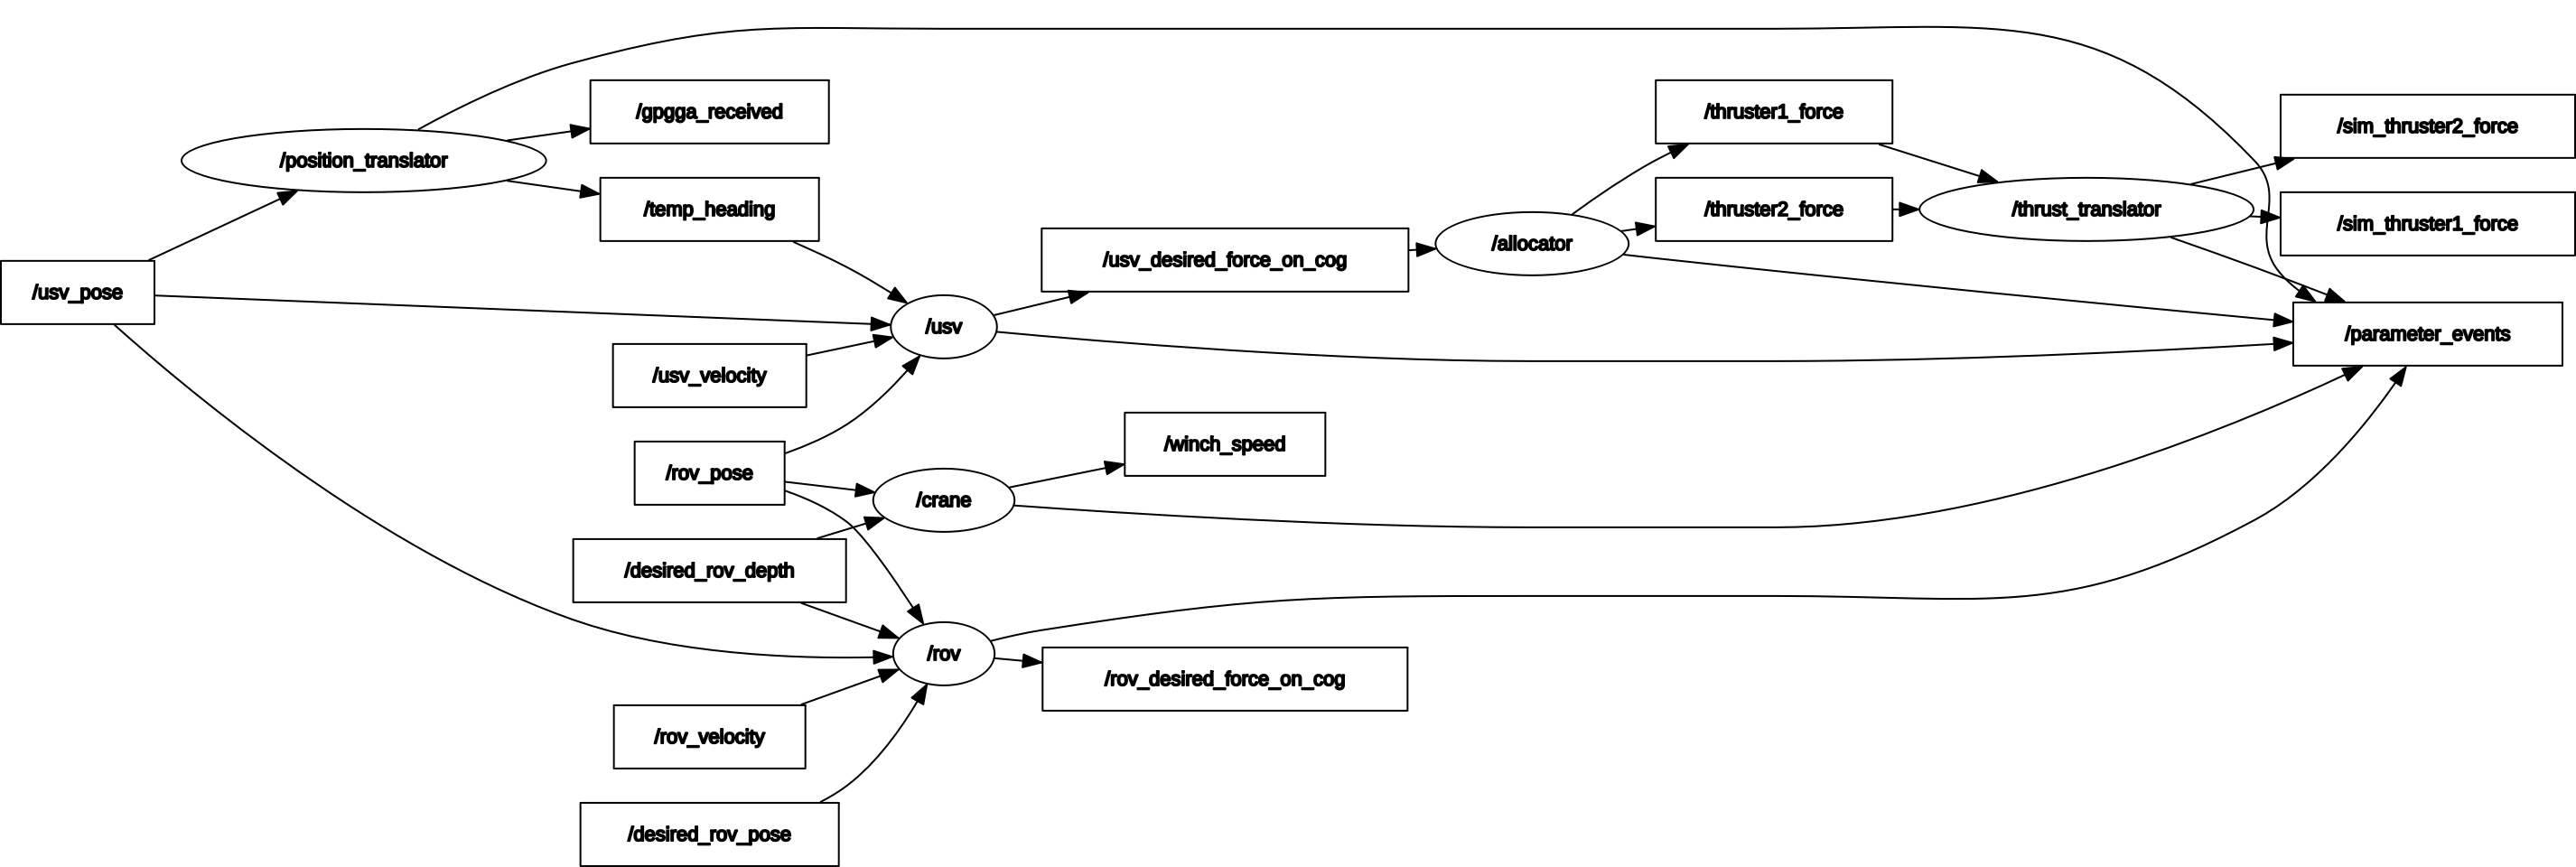
\includegraphics[width=\textheight]{rosgraph-nodata}
    \caption{Graph of the ROS node network without the data collector}
\end{sidewaysfigure}

\begin{sidewaysfigure}
    \centering
    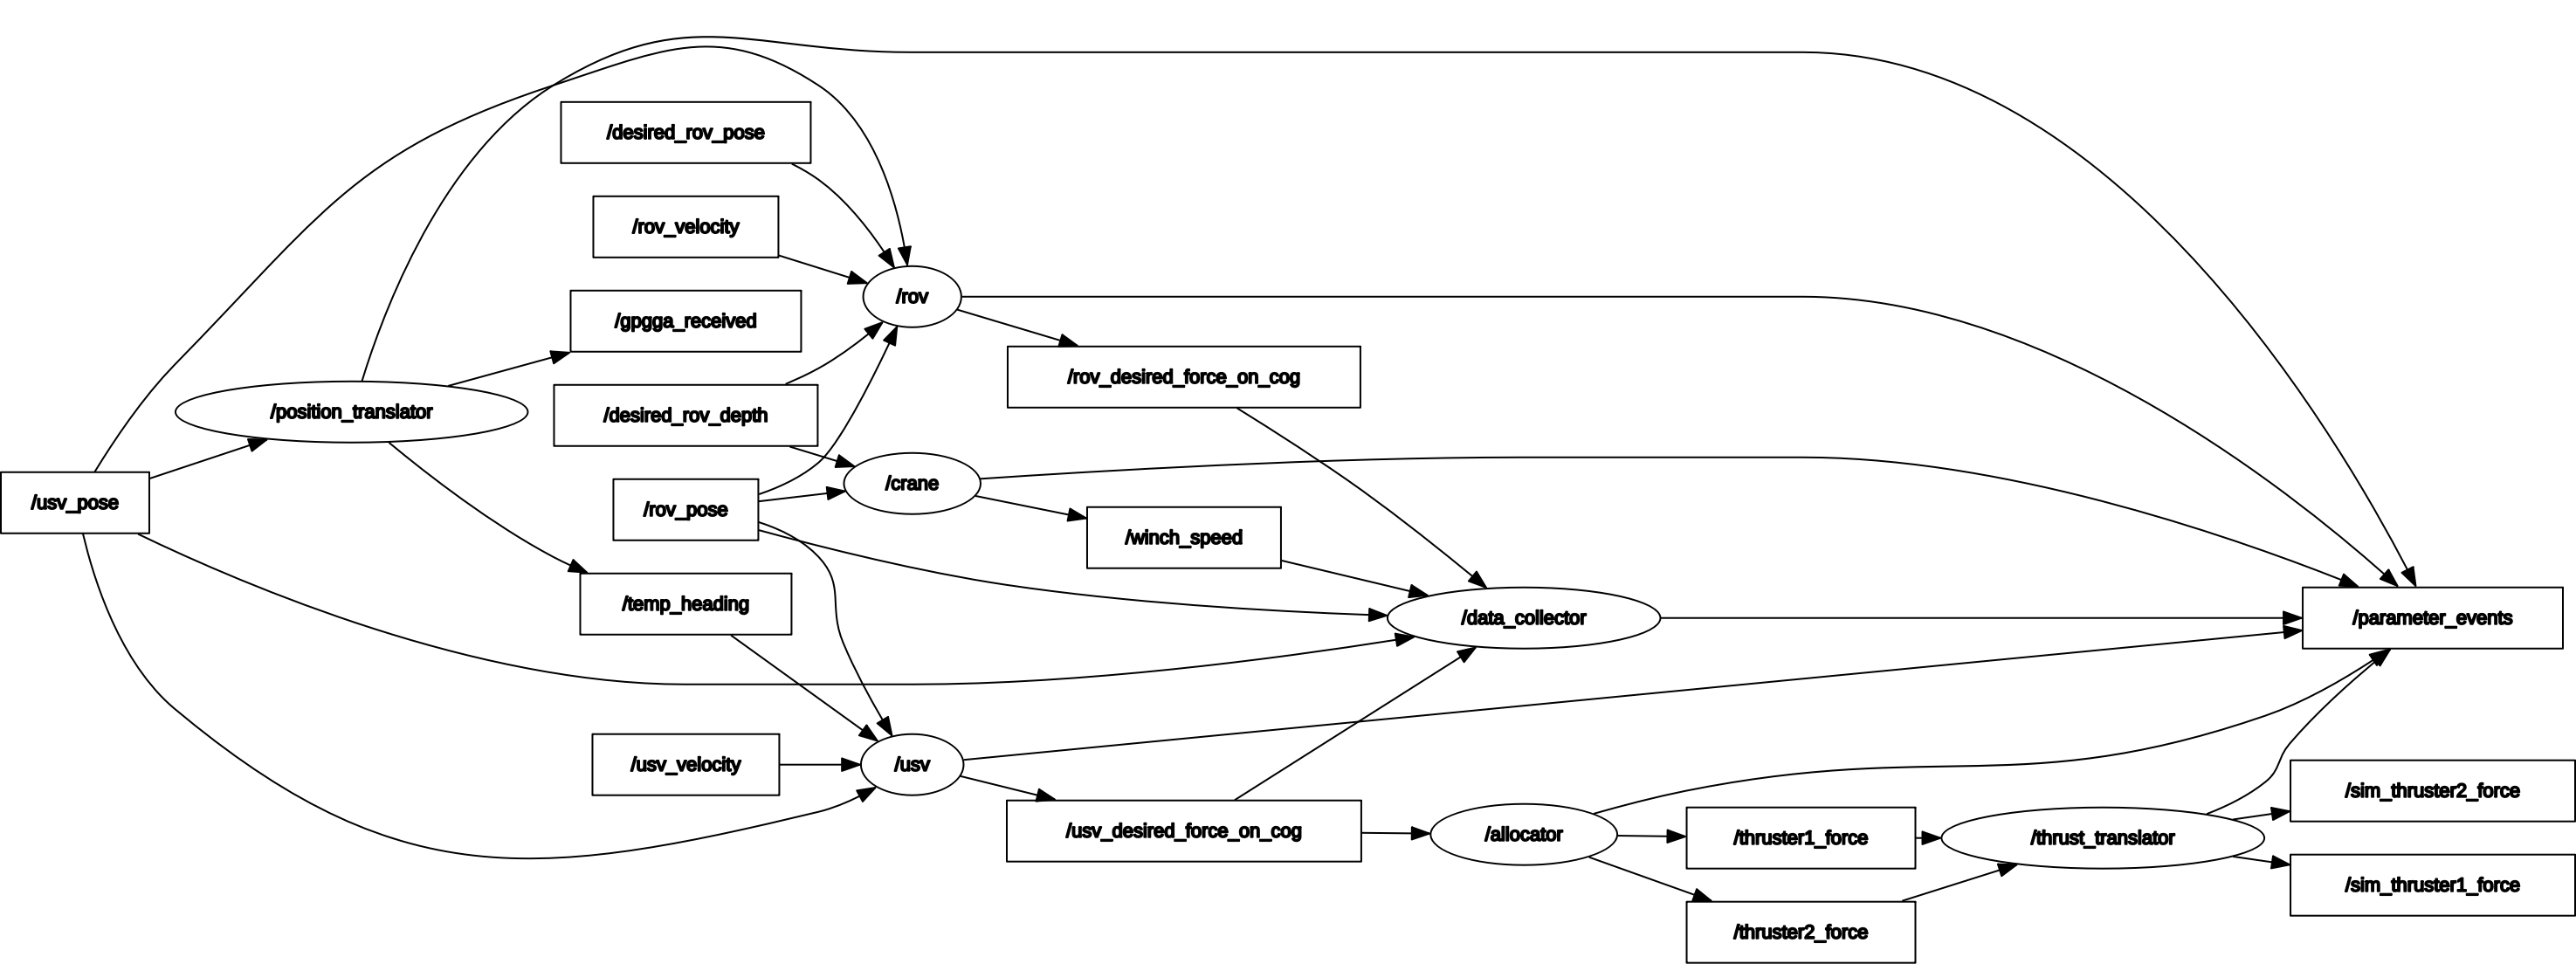
\includegraphics[width=\textheight]{rosgraph-data}
    \caption{Graph of the ROS node network with data collection active}
\end{sidewaysfigure}

\subsection{Future developments}
There is further work necessary on the development front. A functioning human-machine interface is high on the priority list. As shown in \cref{fig:gui}, a non-functioning graphical user interface has been mocked up using the QT framework. Future work would include connecting the GUI to a chart plotter to allow an operator to easily input positions to the system.

While the results show that the control system is working, it is not working very well. The goal of this project has not been to fully develop the control system, but to create the development space to do further development. As it stands, further tuning of the controller parameters is necessary. It is also necessary to find more information on the physical vessel and its capabilities to set the control authority more appropriately. It would also be nice to implement more advanced control functions, such as predictive control based on historical data.











\end{document}
